%!TeX root=main.tex
\begin{section}{Nice Tree Decomposition}
	\label{section:NTD}
	In this section, we'll go over how we converted a tree decomposition into a nice tree decomposition. 
	
	%!TeX root=main.tex

\begin{figure}
	\begin{subfigure}[b]{0.3\textwidth}
		\tikzset{every picture/.style={line width=0.75pt}} %set default line width to 0.75pt        
		\begin{center}	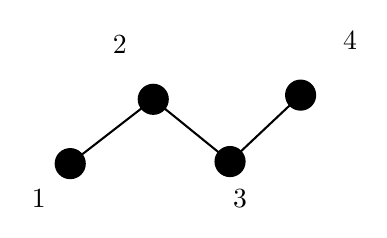
\begin{tikzpicture}[x=0.75pt,y=0.75pt,yscale=-1,xscale=1]
			%uncomment if require: \path (0,753); %set diagram left start at 0, and has height of 753
			
			%Shape: Circle [id:dp38248290994343526] 
			\draw  [fill={rgb, 255:red, 0; green, 0; blue, 0 }  ,fill opacity=1 ] (136,117) .. controls (136,113.13) and (139.13,110) .. (143,110) .. controls (146.87,110) and (150,113.13) .. (150,117) .. controls (150,120.87) and (146.87,124) .. (143,124) .. controls (139.13,124) and (136,120.87) .. (136,117) -- cycle ;
			%Shape: Circle [id:dp2739931949432536] 
			\draw  [fill={rgb, 255:red, 0; green, 0; blue, 0 }  ,fill opacity=1 ] (247,84) .. controls (247,80.13) and (250.13,77) .. (254,77) .. controls (257.87,77) and (261,80.13) .. (261,84) .. controls (261,87.87) and (257.87,91) .. (254,91) .. controls (250.13,91) and (247,87.87) .. (247,84) -- cycle ;
			%Shape: Circle [id:dp6358813933166481] 
			\draw  [fill={rgb, 255:red, 0; green, 0; blue, 0 }  ,fill opacity=1 ] (213,116) .. controls (213,112.13) and (216.13,109) .. (220,109) .. controls (223.87,109) and (227,112.13) .. (227,116) .. controls (227,119.87) and (223.87,123) .. (220,123) .. controls (216.13,123) and (213,119.87) .. (213,116) -- cycle ;
			%Shape: Circle [id:dp48939126493276053] 
			\draw  [fill={rgb, 255:red, 0; green, 0; blue, 0 }  ,fill opacity=1 ] (176,86) .. controls (176,82.13) and (179.13,79) .. (183,79) .. controls (186.87,79) and (190,82.13) .. (190,86) .. controls (190,89.87) and (186.87,93) .. (183,93) .. controls (179.13,93) and (176,89.87) .. (176,86) -- cycle ;
			%Straight Lines [id:da20589949937660657] 
			\draw    (143,117) -- (183,86) ;
			%Straight Lines [id:da9819397938135097] 
			\draw    (220,116) -- (254,84) ;
			%Straight Lines [id:da11052047537584375] 
			\draw    (183,86) -- (220,116) ;
			
			% Text Node
			\draw (123,128) node [anchor=north west][inner sep=0.75pt]   [align=left] {1};
			% Text Node
			\draw (162,54) node [anchor=north west][inner sep=0.75pt]   [align=left] {2};
			% Text Node
			\draw (220,128) node [anchor=north west][inner sep=0.75pt]   [align=left] {3};
			% Text Node
			\draw (273,52) node [anchor=north west][inner sep=0.75pt]   [align=left] {4};
			
			
			\end{tikzpicture}
		\end{center}
		\caption{$\mathcal{P}_4$}
		\label{p4}
	\end{subfigure}
	\begin{subfigure}[b]{0.3\textwidth}
		\begin{center}
			
			\tikzset{every picture/.style={line width=0.75pt}} %set default line width to 0.75pt        
			
			
			\tikzset{every picture/.style={line width=0.75pt}} %set default line width to 0.75pt        
			
			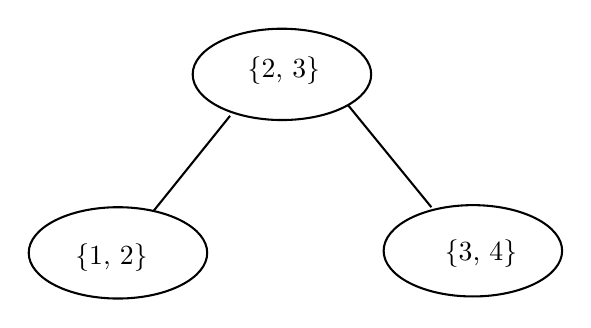
\begin{tikzpicture}[x=0.75pt,y=0.75pt,yscale=-1,xscale=1]
			%uncomment if require: \path (0,632); %set diagram left start at 0, and has height of 632
			
			%Shape: Ellipse [id:dp5175570165318644] 
			\draw   (281,83) .. controls (281,70.85) and (300.25,61) .. (324,61) .. controls (347.75,61) and (367,70.85) .. (367,83) .. controls (367,95.15) and (347.75,105) .. (324,105) .. controls (300.25,105) and (281,95.15) .. (281,83) -- cycle ;
			%Shape: Ellipse [id:dp7529479424703472] 
			\draw   (202,169) .. controls (202,156.85) and (221.25,147) .. (245,147) .. controls (268.75,147) and (288,156.85) .. (288,169) .. controls (288,181.15) and (268.75,191) .. (245,191) .. controls (221.25,191) and (202,181.15) .. (202,169) -- cycle ;
			%Shape: Ellipse [id:dp7057208736562427] 
			\draw   (373,168) .. controls (373,155.85) and (392.25,146) .. (416,146) .. controls (439.75,146) and (459,155.85) .. (459,168) .. controls (459,180.15) and (439.75,190) .. (416,190) .. controls (392.25,190) and (373,180.15) .. (373,168) -- cycle ;
			%Straight Lines [id:da698063510315667] 
			\draw    (299,103) -- (262,149) ;
			%Straight Lines [id:da6342459798451947] 
			\draw    (356,98) -- (396,147) ;
			
			
			% Text Node
			\draw (306,73) node [anchor=north west][inner sep=0.75pt]   [align=left] {\{2, 3\}};
			% Text Node
			\draw (223,163) node [anchor=north west][inner sep=0.75pt]   [align=left] {\{1, 2\}};
			% Text Node
			\draw (401,161) node [anchor=north west][inner sep=0.75pt]   [align=left] {\{3, 4\}};
			
			
			\end{tikzpicture}
		\end{center}
		\caption{Tree Decomposition}
		\label{TreeDecomp}
	\end{subfigure}
\end{figure}

\begin{figure}
	\centering
	
	
	\tikzset{every picture/.style={line width=0.75pt}} %set default line width to 0.75pt        
	
	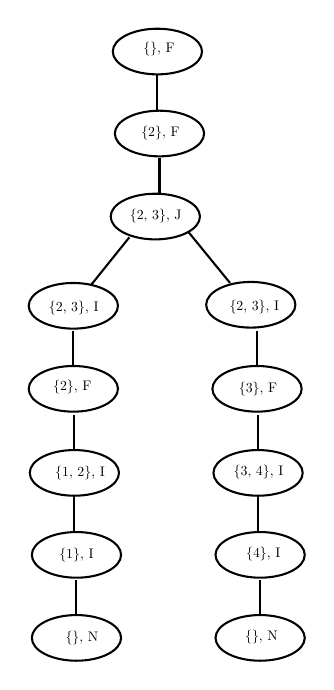
\begin{tikzpicture}[x=0.75pt,y=0.75pt,yscale=-0.5,xscale=0.5, every node/.style={scale=0.5}]
	%uncomment if require: \path (0,770); %set diagram left start at 0, and has height of 770
	
	%Shape: Ellipse [id:dp5248588589594857] 
	\draw   (250,225) .. controls (250,212.85) and (269.25,203) .. (293,203) .. controls (316.75,203) and (336,212.85) .. (336,225) .. controls (336,237.15) and (316.75,247) .. (293,247) .. controls (269.25,247) and (250,237.15) .. (250,225) -- cycle ;
	%Shape: Ellipse [id:dp8855808935720543] 
	\draw   (171,311) .. controls (171,298.85) and (190.25,289) .. (214,289) .. controls (237.75,289) and (257,298.85) .. (257,311) .. controls (257,323.15) and (237.75,333) .. (214,333) .. controls (190.25,333) and (171,323.15) .. (171,311) -- cycle ;
	%Shape: Ellipse [id:dp606634779506167] 
	\draw   (342,310) .. controls (342,297.85) and (361.25,288) .. (385,288) .. controls (408.75,288) and (428,297.85) .. (428,310) .. controls (428,322.15) and (408.75,332) .. (385,332) .. controls (361.25,332) and (342,322.15) .. (342,310) -- cycle ;
	%Straight Lines [id:da06110450839607107] 
	\draw    (268,245) -- (231,291) ;
	%Straight Lines [id:da47523090776105303] 
	\draw    (325,240) -- (365,289) ;
	%Shape: Ellipse [id:dp20858809529480138] 
	\draw   (348,391) .. controls (348,378.85) and (367.25,369) .. (391,369) .. controls (414.75,369) and (434,378.85) .. (434,391) .. controls (434,403.15) and (414.75,413) .. (391,413) .. controls (367.25,413) and (348,403.15) .. (348,391) -- cycle ;
	%Straight Lines [id:da02966169889332848] 
	\draw    (391,369) -- (391,335) ;
	%Shape: Ellipse [id:dp24948535115685688] 
	\draw   (349,472) .. controls (349,459.85) and (368.25,450) .. (392,450) .. controls (415.75,450) and (435,459.85) .. (435,472) .. controls (435,484.15) and (415.75,494) .. (392,494) .. controls (368.25,494) and (349,484.15) .. (349,472) -- cycle ;
	%Straight Lines [id:da8483719242560979] 
	\draw    (392,450) -- (392,416) ;
	%Shape: Ellipse [id:dp3104496219770304] 
	\draw   (351,551) .. controls (351,538.85) and (370.25,529) .. (394,529) .. controls (417.75,529) and (437,538.85) .. (437,551) .. controls (437,563.15) and (417.75,573) .. (394,573) .. controls (370.25,573) and (351,563.15) .. (351,551) -- cycle ;
	%Straight Lines [id:da6840204738433688] 
	\draw    (392,528) -- (392,494) ;
	%Shape: Ellipse [id:dp16734206164466903] 
	\draw   (351,631) .. controls (351,618.85) and (370.25,609) .. (394,609) .. controls (417.75,609) and (437,618.85) .. (437,631) .. controls (437,643.15) and (417.75,653) .. (394,653) .. controls (370.25,653) and (351,643.15) .. (351,631) -- cycle ;
	%Straight Lines [id:da7490825803812134] 
	\draw    (394,609) -- (394,575) ;
	%Shape: Ellipse [id:dp625252921606493] 
	\draw   (171,391) .. controls (171,378.85) and (190.25,369) .. (214,369) .. controls (237.75,369) and (257,378.85) .. (257,391) .. controls (257,403.15) and (237.75,413) .. (214,413) .. controls (190.25,413) and (171,403.15) .. (171,391) -- cycle ;
	%Straight Lines [id:da8747789462467919] 
	\draw    (214,369) -- (214,335) ;
	%Shape: Ellipse [id:dp7167438998112289] 
	\draw   (172,472) .. controls (172,459.85) and (191.25,450) .. (215,450) .. controls (238.75,450) and (258,459.85) .. (258,472) .. controls (258,484.15) and (238.75,494) .. (215,494) .. controls (191.25,494) and (172,484.15) .. (172,472) -- cycle ;
	%Straight Lines [id:da6775872899017072] 
	\draw    (215,450) -- (215,416) ;
	%Shape: Ellipse [id:dp4830312977183936] 
	\draw   (174,551) .. controls (174,538.85) and (193.25,529) .. (217,529) .. controls (240.75,529) and (260,538.85) .. (260,551) .. controls (260,563.15) and (240.75,573) .. (217,573) .. controls (193.25,573) and (174,563.15) .. (174,551) -- cycle ;
	%Straight Lines [id:da9065403939161113] 
	\draw    (215,528) -- (215,494) ;
	%Shape: Ellipse [id:dp7622433258791789] 
	\draw   (174,631) .. controls (174,618.85) and (193.25,609) .. (217,609) .. controls (240.75,609) and (260,618.85) .. (260,631) .. controls (260,643.15) and (240.75,653) .. (217,653) .. controls (193.25,653) and (174,643.15) .. (174,631) -- cycle ;
	%Straight Lines [id:da5159274806843283] 
	\draw    (217,609) -- (217,575) ;
	%Shape: Ellipse [id:dp36642109285923596] 
	\draw   (252,66) .. controls (252,53.85) and (271.25,44) .. (295,44) .. controls (318.75,44) and (338,53.85) .. (338,66) .. controls (338,78.15) and (318.75,88) .. (295,88) .. controls (271.25,88) and (252,78.15) .. (252,66) -- cycle ;
	%Shape: Ellipse [id:dp579170044821565] 
	\draw   (254,145) .. controls (254,132.85) and (273.25,123) .. (297,123) .. controls (320.75,123) and (340,132.85) .. (340,145) .. controls (340,157.15) and (320.75,167) .. (297,167) .. controls (273.25,167) and (254,157.15) .. (254,145) -- cycle ;
	%Straight Lines [id:da11334735837963827] 
	\draw    (295,122) -- (295,88) ;
	%Straight Lines [id:da07305489134692822] 
	\draw    (297,203) -- (297,169) ;
	
	
	% Text Node
	\draw (278,136) node [anchor=north west][inner sep=0.75pt]   [align=left] {\{2\}, F};
	% Text Node
	\draw (280,55) node [anchor=north west][inner sep=0.75pt]   [align=left] {\{\}, F};
	% Text Node
	\draw (267,216) node [anchor=north west][inner sep=0.75pt]   [align=left] {\{2, 3\}, J};
	% Text Node
	\draw (189,305) node [anchor=north west][inner sep=0.75pt]   [align=left] {\{2, 3\}, I};
	% Text Node
	\draw (363,304) node [anchor=north west][inner sep=0.75pt]   [align=left] {\{2, 3\}, I};
	% Text Node
	\draw (195,464) node [anchor=north west][inner sep=0.75pt]   [align=left] {\{1, 2\}, I};
	% Text Node
	\draw (199,543) node [anchor=north west][inner sep=0.75pt]   [align=left] {\{1\}, I};
	% Text Node
	\draw (205,623) node [anchor=north west][inner sep=0.75pt]   [align=left] {\{\}, N};
	% Text Node
	\draw (378,622) node [anchor=north west][inner sep=0.75pt]   [align=left] {\{\}, N};
	% Text Node
	\draw (379,542) node [anchor=north west][inner sep=0.75pt]   [align=left] {\{4\}, I};
	% Text Node
	\draw (367,463) node [anchor=north west][inner sep=0.75pt]   [align=left] {\{3, 4\}, I};
	% Text Node
	\draw (193,381) node [anchor=north west][inner sep=0.75pt]   [align=left] {\{2\}, F};
	% Text Node
	\draw (372,383) node [anchor=north west][inner sep=0.75pt]   [align=left] {\{3\}, F};
	
	
	\end{tikzpicture}
	\caption{Nice Tree Decomposition of tree in Fig. \ref{TreeDecomp}}
	\label{NiceTreeDecomposition}
\end{figure}
	
	The idea that we keep the nodes which are in the tree decomposition as is, and insert new nodes in between the older nodes in order to ``smoothen" the change from one node to another. 
	
	\begin{subsection}{Join Nodes}
			If a node has multiple children ($c$), we have to create join nodes. An easy way to do so is to duplicate the current node, add those two duplicates as children to the current node and then assign the first child to the left duplicated node. Now, we have $c-1$ children left, and we recurse on the right duplicated child. The current node is a join node. \\
			
			This procedure increases the height of the tree by $c$ if the original node had $c$ children. This is because we keep adding vertices only to the right. However, it doesn't matter as the algorithm does not depend on the depth. However if we did, we could minimise the height by making the binary tree of joined nodes balanced. \\
			
			We can refer to the example in Fig. \ref{TreeDecomp} where the node $\{2, 3\}$ has been duplicated as shown in Fig. \ref{NiceTreeDecomposition}. To make the tree nice w.r.t the duplicated node and its child, we'll go to the next subsection .
	\end{subsection}

	\begin{subsection}{Introduce and Forget Nodes}
		At this point, any node which has child with a different bag of vertices has only one child. By making the transition for that nice, we end up making the entire tree nice. \\
		
		Given nodes $X$ and $Y$, where $Y$ is the only child of $X$, we want to insert nodes between $X$ and $Y$ such that there is a nice path from $Y$ to $X$ as we go up the tree. \\
		
		To compute this, while going from $Y \rightarrow X$, we should add forget nodes for all vertices in $Y \backslash X$ and then add introduce nodes for all vertices in $X \backslash Y$. Note that this order is important. If we reverse the order, we can potentially increase the treewidth. \\ 
		
		This has been done in Fig. \ref{NiceTreeDecomposition} where we go from $\{3, 4\} \rightarrow \{2, 3\}$ in this manner. 
	\end{subsection}

	\begin{subsection}{Introduce Edge Nodes}
		After applying the above steps, we get a nice tree decomposition which adds and forgets vertices one by one. If we would like to add edges one by one as well, 
		Given an edge containing two vertices $u$ and $v$, let $f(u)$ and $f(v)$ denote the nodes where $u$ and $v$ are forgotten. Let $T_u$ and $T_v$ denote the subtrees of the tree decomposition rooted at $f(u)$ and $f(v)$ respectively. Now, it's easy to see that either $T_u \subset T_v$ or $T_v \subset T_u$ where $\subset$ denotes the ``subtree" property. If it isn't, then there is no node in common between $T_u$ and $T_v$ and that contradicts the property that there exists a bag containing $u$ and $v$ if there is an edge $(u, v)$ in the graph. 
		
		In such a scenario, without loss of generality, assume $T_v \subset T_u$. Then, we add an Introduce Edge node just before $v$ is forgotten, i.e. as a child of $f(v)$. This ensures that the graph isn't joined and the edge is only introduced once.  
	\end{subsection}
\end{section}


